\section{Introduction}

During this group computing project, our team has implemented a \py{} package for Moment Expansion Approximation iNference and Simulation, \means{} for short. 
The development process and the results have been described in detail in the main group report, which I am not going to reiterate here.

Instead, in this document, I attempt to summarise my major contributions to \means{}, and justify certain decisions as well as share my views on the software engineering process.

I start by providing some anecdotal evidence on how advanced software engineering techniques helped us to succeed in this project. 
I then list the contributions to the source code I felt were noteworthy. Then I briefly cover the pipeline functionality implemented in \means{} that we deliberately omitted from the group report.
After that, I briefly reiterate the results described in the main report and provide the additional data.
Finally, I conclude the report by providing a retrospect and considering directions for future work.

\section{Software Development Process}

In the modern day, when computers are becoming the driving force of innovation and progress, the whole world is facing the need to either adjust to this computerisation or risk to be left behind by others.
Naturally, software is becoming critically important for scientific communities. This importance raises the demand for scientists who are also proficient in computer programming. Unfortunately, while knowledge of computer programming is deemed critical, the necessity to study software engineering is still being debated. 

The common argument against the need to study software engineering states that people often care only about the end result, and not how it was obtained or how easy-to-read code is.
This reasoning seems to be ironic to me as the same argument can be used to describe why the software-engineering methodologies emerged in the first place. 
For instance, two of the main principles of the \emph{agile} methodology\cite{_manifesto_????} treat the ``working software as the primary measure of success" and claim that ``simplicity -- the art of maximising of work \emph{not} done -- is essential"\cite{paulk_agile_2002}. 
In fact \emph{agile} methodology is often viewed as an alternative to the approaches that aim to create this idealistic, properly structured and well-documented software, such as the traditional \emph{waterfall} model.

It was my personal goal, and I believe my biggest contribution, to share my experience in software engineering in order to incorporate the \emph{agile} methodology into our development cycle. 
In this project I aimed to introduce my peers to concepts that might have not been known to them previously as well as to try to promote them. 
This section lists a couple of the modern software development practices we aimed to employ, and provides a short description of how they contributed to the success of \means{}.

Whenever I introduced a concept to the peers, regardless if they have heard it before or not, I also tried to push it to further to the limits, so the biggest advantage can be seen. 
For instance, not only we were using \verb"git"\cite{git} for our version control, but we were also using appropriate branching workflow. 
This allowed each one of us to work on separate things in isolation, and ensured one's changes will not break the other's work. 
In turn this provided the courage for us to be able to experiment with the code more, knowing these experiments will not impact others.
Without this courage, performance improvements described in the group report's section \autoref*{GR:performance} may have never been made.

Another factor that contributed to the ability to change the key parts of the system without the fear of breaking something was the early incorporation of automated tests to the system. 
This created a way to validate the correctness of our software quickly.
Similarly, it allowed us to pin-point the location of a failure quickly, minutes after it occurred.
In turn it allowed us to spend less time testing our software, but trust it more.
This has had a positive effect on our confidence in the validity of the observations made (as described in the \autoref*{GR:results} of group report). Our approach to software testing is summarised in the main report's \autoref*{GR:sec:testing}.

To help ourselves \emph{increase the amount of work not done}, we set up a continuous integration server.
This server, implemented by the \emph{Jenkins CI} platform\cite{_jenkins_????}, has responsibly been running every single test we have after every push to the central code repository we made. 
We assumed that if the code does not work on \emph{Jenkins}, as we called it, it does not work at all, regardless of whether the code works on the author's machine or not. 
Such code could then be retracted, fixed and pushed again to the main repository, at which point it will be tested again. 
This way we reduced the number of issues that occurred due to simple human error, such as files missing from the central repository, or tests not run before a commit.

Similarly, \emph{Jenkins} enabled us to run code in different environments. For instance, we kept all the libraries updated to the latest version in one of the environments we ran the code on. 
It was because of this special environment that we spotted an incompatibility with the latest version of \verb"Assimulo"\cite{andersson_christian_assimulo:_????} -- the package providing ODE solver implementations in \py{} -- minutes after that version became public. We were then able to prove that this incompatibility was a problem with the \verb"Assimulo" package, not ours. 
We then worked together with Cristian Andersson (one of the developers of \verb"Assimulo") to it get fixed and new version of the package released.
In the sense, this continuous integration environment has contributed to two projects -- \verb"Assimulo" and \means{} -- as if not for it, said bug in the library might still be present today.

Finally, I explained in detail the advanced concepts of Object-Oriented Programming, such as inheritance and encapsulation to my peers so they could be applied in our project.
I attempted to show how these concepts make the code both easier to maintain, and easier to write in the first place, hopefully allowing the peers to transfer these skills to their other projects as well.
In the end, I believe we have succeeded at creating a highly modular codebase, which should be easy to maintain in the future. The summary of our code base is available in the \autoref*{GR:sec:package} of the group report, as well as in the documentation, described in the appendix \autoref*{GR:sec:documentation} of group report.

Besides the programming-related best practices of software engineering, we also implemented certain project management aspects suggested by \emph{agile} methodologies. 
For instance, we structured our work into weekly iterations. We were planning the things we need to do for the week, and reviewing the things we have done at the end of it. 
We have structured our iterations to end just before the weekly meetings with supervisors, so we could also immediately get the feedback.
This allowed to keep the project on a clear track, going the right way and within the scope required.

In the end, I believe that the software-engineering approaches I described above acted both as an educational exercise and a way to be more efficient, when it comes to software development.
I strongly believe that without them, we would not have been able to progress as much with the project as we did.
I also hope that the anecdotal evidence listed above may serve as a proof of utility of software engineering approaches, however small, and maybe act as an argument in favour of a need to study it.

\section{Significant Code Contributions}

In the previous section I have talked about the software development process in general and my contributions to it. 
Below I list my most noteworthy contributions to the source code of \means{}.

\subsection{Design of Interface for Simulation}
\label{sec:simulation}

It is no secret that we did not start this project from scratch.
The previous year's MSc students have already contributed a large quantity of \py{} code that provided some basic functionality of \means{}. In this project, we attempted to simplify this functionality and therefore make it easier to use and maintain (see \autoref*{GR:sec:aims_of_the_project} in the group report).
To do this, we reviewed the code and noted the parts of it that we felt needed to be changed. 
We then approached these parts, one by one, and refactored them in isolation, aiming not to break the remaining parts of the system.

I have worked on the simplifications of simulation mechanism implemented in the previous year's version of the code. 
In a nutshell, this original mechanism split the process into three parts: the \python{} code was transcribed of into C code that interacts with the \verb"CVODE" library\cite{hindmarsh_sundials_2005}, which then was then compiled, and later on run directly from \py{}.

We felt that his rather \emph{ad-hoc} process of transcribing \py{} to C seemed to be error prone and unnatural. 
Similarly, \py{} code was interacting with the compiled C library in a platform-specific and multiprocess-incompatible way, reducing the portability and possible uses of the code. In our view, these two factors justified the need to replace this system.

We found \verb"Assimulo" -- a package already mentioned once before in this report -- to be a suitable replacement for the wrappers around \verb"CVODE" that would allow us to easily extend the functionality as well. 
I have prototyped and implemented the code change replacing the mechanism described above with a cleaner mechanism offered by the \verb"Assimulo" package. This also allowed us to add the sensitivity analysis support to the \means{} package as well as the ability to run the simulations using a different \gls{ode} solver.
This new interface is further described in detail in \autoref*{GR:sec:package_structure:simulation} and demonstrated in\autoref*{GR:sec:simulation} of the main report.

While \verb"Assimulo" handled much of the heavy-lifting when it comes to solving \glspl{ode}, we still needed to increase the performance of the numeric evaluations of the symbolic expressions. 
Previously this was a non-issue as these expressions were transcribed to C. 
Luckily, \verb"sympy" -- the python package for symbolic mathematics -- has already implemented a collection of methods of evaluating these expressions efficiently. QG and I benchmarked the \verb"lambdify" method, that turns the numeric expression into a \verb"lambda" function, and the  \verb"autowrap" module which compiles the numeric expressions to C.
We did not test the third option -- Theano\cite{bergstra_theano:_2010} -- available in the latest version of \verb"sympy", because the college environment did not support it at that time\footnote{We eventually updated the college environment to run the latest version of the package, however we did not get back to this benchmark due to the time constraints.}.

\begin{table}
    \centering
    \begin{tabular}{l|l}
    Method & Runtime \\
    \hline
    Default & 628 microseconds \\
    \verb"lambdify" & 10.7 microseconds \\
    \verb"autowrap" & 2.89 microseconds \\
    Theano & not measured \\
    \end{tabular}
    \caption{Results of the three out of four numeric evaluation methods available in {\tt sympy}. 
    The results were recorded using the {\tt \%timeit} 
    function provided by IPython\cite{perez_ipython:_2007} interactive environment. 
    This function performs as many evaluations of the code it can fit in 2 seconds and returns the best runtime of all the repetitions.
    The evaluations were performed on the two right-hand-side equations resulting from approximating the dimerisation model up to the moment order of two.
    It is clear from the data that{\tt autowrap} method is a clear winner. 
    Theano performance was not tested as it was not supported in the college environment at the time we performed this test.}
    \label{tab:numeric-runtimes}
\end{table}

The benchmarking results from the experiment are summarised in \autoref{tab:numeric-runtimes}. 
We can see that \verb"autowrap" is clear winner in the benchmark and therefore was chosen to be implemented in our package.
This has proven to be an efficient-enough solution for most of the day-to-day needs, becoming an issue only for high-maximal order moment closures, where the number of expressions to evaluate is large.

In the future, however, it would be interesting to benchmark the Theano performance, whose inherent GPU support could speed up the evaluations even more.
Particularly, I believe it would help to reduce the exponential slope of runtime arising from the exponential increase of the number of equations as the maximal moment order is increased (see \autoref{GR:fig:solver-runtimes} in the group report) to make the simulations feasible for even more complicated systems.

\subsection{Design of Interface for Parameter Inference}

Besides refactoring the simulation mechanisms from the previous year's code, I have also worked on restructuring the parameter inference interface. 
The original interface, while fully working, was split into two distinct, but very similar parts: sum-of-square distance based inference, and parametric distance based inference. Similarly, the specification of inference parameters seemed slightly convoluted and not suitable to be used from an interactive interface. 

During the iterations of this project both of these issues were removed. The new interface for parameter inference is
both unified and more succinct as the previous one. This new interface is demonstrated in \autoref*{GR:sec:parameter_inference} of the group report.

Additionally, this refactoring enabled our users to design their own distance functions, as demonstrated in \autoref*{GR:sec:distance_measures} of the group report.
Finally, by the end of the project, SF and I have added additional plotting functionality for the parameter inference results, such as the contour plot of the distance landscape, as illustrated in 
\autoref*{GR:sec:investigating_distance_landscape} of the group report, which we believe will aid the future users in exploring their data.

\subsection{Pipeline Support}

During the final days of this project, when we were generating the figures for the results section in the group report (\autoref{GR:results}), we realised that the scale of these figures was quickly becoming hard to manage. 
At this point each one of us has had already written a couple of lines of boilerplate code that performs the \acrlong{mea}, stores the result,  has a loop through simulation or parameter inference procedures on this result, and stores the final results to different file.

Since each one of us had their own version of the same code, we were deemed to repeat the mistakes of each other. 
Tasks that were supposed to be running overnight, failed early. Resulting data was not saved correctly, rendering it unreadable.
Similarly, we were unlikely to collaborate and share the results with each other, as they were all stored in different formats.
We needed something to manage these processes better and prevent the issues from reoccurring.

I proposed to use \verb"luigi"\cite{_luigi_????} -- a \python{} library developed by the engineers in \emph{Spotify} -- to provide an unified framework for the common tasks we had to do. 
This package allows to break down complicated tasks into a set of smaller ones and specify the interdependencies between them.
The system is then allowed to perform these tasks in any order, often in parallel, as long as all of the tasks are executed after their children in the dependancy tree are.
This is exactly the same concept as the one implemented by \emph{GNU Make}\cite{gnumake}, for those who are familiar with it. Unlike \emph{Make}, however, \verb"luigi" package has a full support for parametric tasks. Also, integration with \verb"luigi" is easier as it is written in \python{}.

I wrote the general wrappers around the means code in the \verb"luigi" framework. 
For instance, I implemented the \verb"MEATask" objects that would take a model, \gls{maxord}, closure method as a parameter and return the resulting set of equations corresponding to \gls{mea} approximation requested. 
Another task, \verb"TrajectoryTask", would then treat this task as a dependency and use the set of equations generated to simulate the behaviour of the system. 
A set of such tasks could then be compiled into figures, and figures into documents, the process which is illustrated in \autoref{fig:pipes_example}.

The hierarchical nature of these dependancies is hard to visualise (\autoref{fig:pipes_example}), let alone to implement efficiently.
Using {\tt luigi} package not only allowed us to skip the implementation step for dependancy management, but also allowed to be more flexible in terms of our data. In essence, we were only specifying how to draw the plots, and not how to obtain the data for them.

\begin{figure}
    \centering
     \begin{subfigure}[t]{0.3\textwidth}
        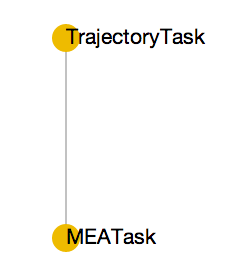
\includegraphics[scale=0.7]{images/TrajectoryTask.png}
        \caption{Dependancies of {\tt TrajectoryTask}}
        \label{fig:pipes_example:TrajectoryTask}
    \end{subfigure}
    ~
    \begin{subfigure}[t]{\textwidth}
        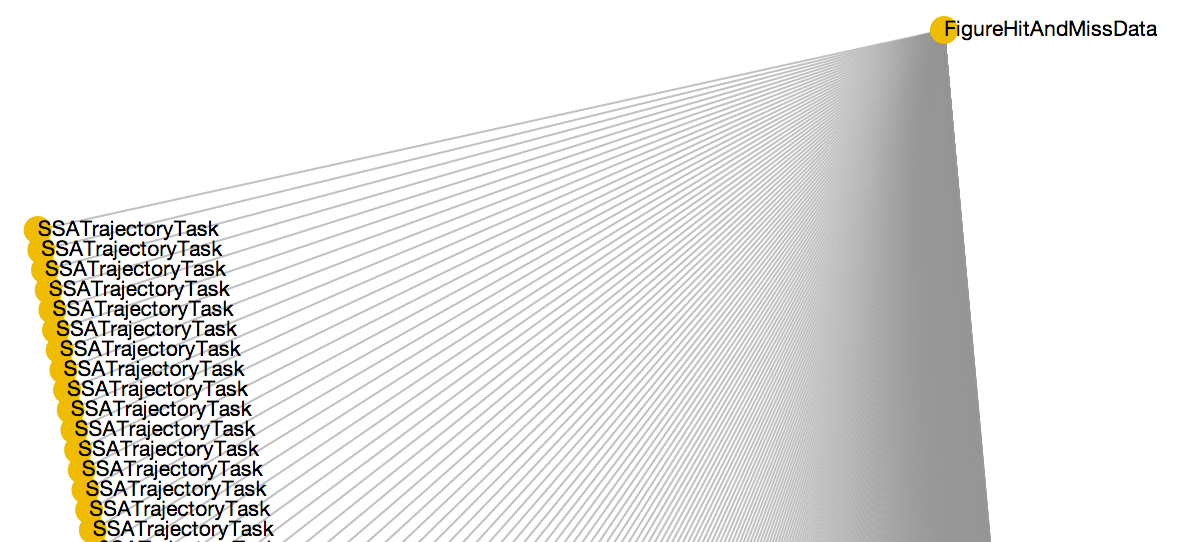
\includegraphics[width=\textwidth]{images/FigureHitAndMissData}
        \caption{Partial dependancies of the data preprocessing step.}
        \label{fig:pipes_example:FigureHitAndMissData}
    \end{subfigure}
    ~
    \begin{subfigure}[t]{\textwidth}
        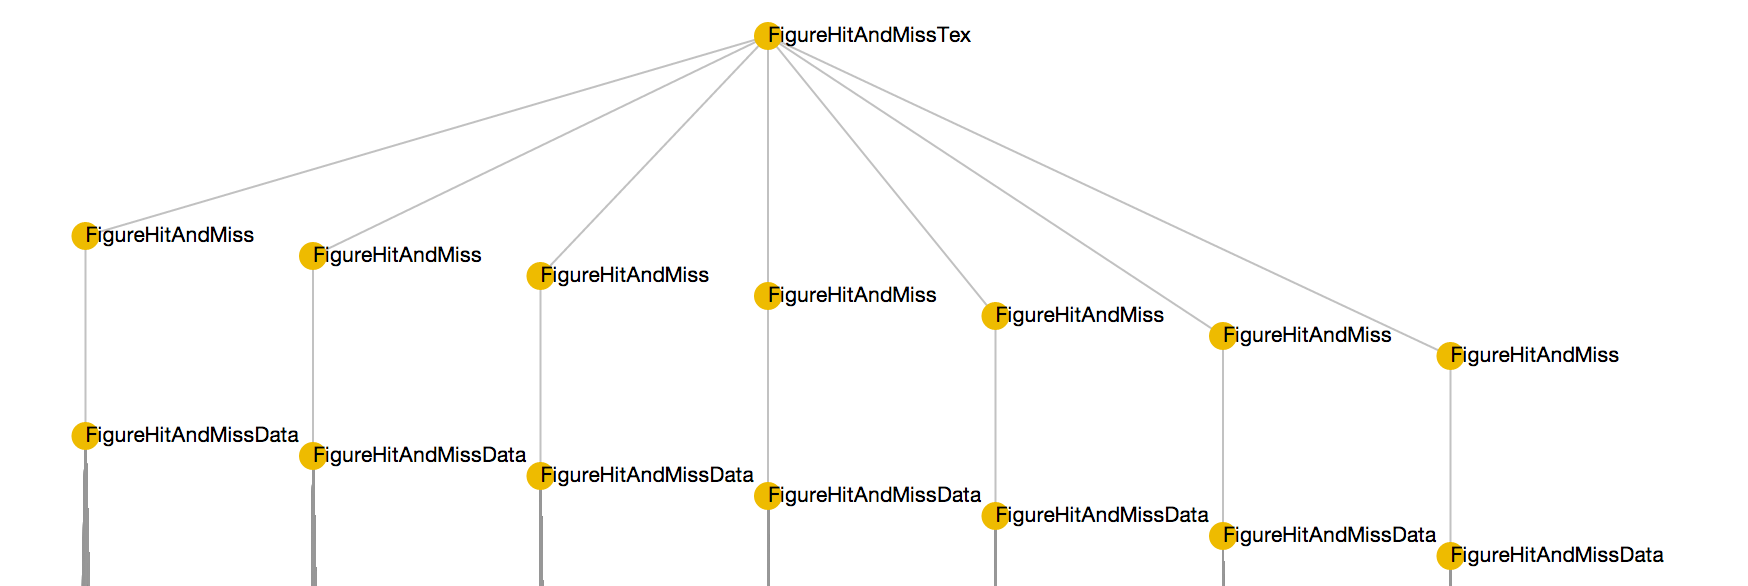
\includegraphics[width=\textwidth]{images/FigureHitAndMissTex.png}
        \caption{Compilation of the data preprocessing tasks into sets of contour plots to be directly embedded to the report.}
        \label{fig:pipes_example:FigureHitAndMissTex}
    \end{subfigure}
    \caption{\emph{Graphical representation of the dependancies between the tasks used to generate the contour plots of solver performance, i.e. the figures in the appendix \autoref{sec:supplementary_figures}.}\\ 
    Each  \texttt{TrajectoryTask} depends on \texttt{MEATask} (\ref{fig:pipes_example:TrajectoryTask}).
    A number of these tasks, one for each point of the parameter space, is required to compile the grid of we want to plot as a contour plot.
    Besides the regular trajectories, one trajectory per parameter space obtained using \acrlong{ssa} was also needed (\ref{fig:pipes_example:FigureHitAndMissData}).
    The obtained trajectories can then be used to compute the distance grid, and these grids could be drawn as contour plots and compiled together into \LaTeX{} figures (\ref{fig:pipes_example:FigureHitAndMissTex}), resulting into figures similar to the ones in the appendix \autoref{sec:supplementary_figures}.\\
    For simplicity of visualisation, only the partial picture has been drawn.\\
    NB: The name {\tt FigureHitAndMiss} comes from the earlier iteration of this figure that only marked the points for which the solver has failed, somewhat resembling a target with bullet holes.}
    \label{fig:pipes_example}
\end{figure}

\section{Investigation of \acrshort{mea} Accuracy and Solver Performance}

The pipelines described above were most useful in writing the \emph{results} section of the group report. In my section of this report, \autoref{GR:sec:hit-and-miss}, I worked on generalising the results obtained by QG that he describes in the preceding section of the group report. 
Here I was interested to see how the results change depending on the region of parameter space, as well as the impact different \gls{ode} solvers make on these results.

Due to the short time constraints we had and potentially long runtimes of needed to generate that much data, I have limited myself to only studying a small region of parameter space of the \pft{} model, and the behaviour of only four solvers: \texttt{ode15s}, \texttt{euler}, \texttt{dopri5} and \texttt{rodas}.

Data has shown that certain regions of the parameter space were easier to approximate than others, while other regions of parameter space seemed to be particularly troublesome for the solvers. 
These results are discussed in full in the section \autoref*{GR:sec:hit-and-miss} of the main report.

I also found that there was little difference between the behaviour of different solvers as they all were handling the easy-to-simulate regions well, but failed for the hard ones.
The full set of results for all solvers was not included to the main report, but are attached to the appendix \autoref{sec:supplementary_figures} of this document.

In conclusion, these results show that the accuracy of \gls{mea} for a single parameter set must be taken with a caution. These results suggest that accuracy depends strongly on the region of the parameter space and cannot be generalised from a single point to the entire space, however some general patterns described in \autoref*{GR:sec:hit-and-miss} of the main report can still be observed.

\section{Conclusion}

In this report I aimed to summarise the value I brought to the team during the course of this project.
These contributions included the push towards using advanced software-engineering techniques as well as direct contributions to the codebase such as the design of interfaces for simulation and inference.
I have also suggested using \verb"luigi" framework to produce figures based on data in a pragmatical manner and
used it to analyse MEA performance for a region of parameter space.

Objectively, I believe our team achieved impressive results.
However, due to the fixed timescale, we had to stop exploring somewhere.

As described in \autoref{sec:simulation}, it would be interesting to attempt using Theano for numeric evaluations of symbolic expressions.
If this library is able to give a significant boost to the runtime of the simulations, it might enable the exploration of \gls{mea} for even more complicated systems.

Similarly, it would be interesting to explore the performance of \gls{mea} on a larger parameter space. Why certain regions of this parameter space are easier to model, whilst others show opposite behaviour remains an open question.
Also, we do not how common these regions are, or what their distributions in parameter space are.

In my opinion, answers to these questions will determine the future of \gls{mea}, and, by extension, the adoption of \means.
With the previous tools, we would not have been able to ask these questions as they would have been either too tedious or to slow to answer.
The layer of software we have produced made it simple to address all questions our imagination could raise, making me proud to have taken part in its development.